\chapter{Evaluation}
\label{chp:ch5-evaluation}

\begin{table*}
  \small
  \begin{center}
  \begin{tabular}{ l r r r r r r }
  \toprule
  Benchmark     & CPython3  & CPython  & Jython  & PyPy     & PyPy3    & ZipPy \\
  \midrule
  \textsf{binarytrees}   & $5.40$    & $5.10$   & $10.76$ & $14.05$  & $14.60$  & $39.49$ \\
  \textsf{fannkuchredux} & $2.27$    & $2.20$   & $1.17$  & $101.24$ & $107.52$ & $198.94$ \\
  \textsf{fasta}         & $15.52$   & $16.20$  & $24.13$ & $182.09$ & $174.55$ & $241.76$ \\
  \textsf{mandelbrot}    & $9.00$    & $9.70$   & $3.03$  & $98.15$  & $97.35$  & $105.18$ \\
  \textsf{meteor}        & $100.55$  & $102.83$ & $77.14$ & $265.43$ & $263.75$ & $213.77$ \\
  \textsf{nbody}         & $10.12$   & $9.87$   & $7.40$  & $122.83$ & $122.07$ & $62.42$ \\
  \textsf{pidigits}      & $77.02$   & $77.40$  & $47.59$ & $75.25$  & $73.02$  & $46.59$ \\
  \textsf{spectralnorm}  & $0.90$    & $1.20$   & $1.70$  & $114.60$ & $114.52$ & $115.29$ \\
  \textsf{float}         & $10.82$   & $10.23$  & $11.37$ & $93.57$  & $93.82$  & $191.68$ \\
  \textsf{richards}      & $16.77$   & $15.83$  & $20.35$ & $495.38$ & $490.70$ & $840.93$ \\
  \textsf{chaos}         & $2.05$    & $2.40$   & $3.17$  & $83.77$  & $52.65$  & $139.94$ \\
  \textsf{deltablue}     & $19.62$   & $16.77$  & $26.19$ & $590.25$ & $571.82$ & $460.37$ \\
  \textsf{go}            & $23.15$   & $24.97$  & $46.16$ & $157.29$ & $154.07$ & $356.80$ \\
  \bottomrule
  \end{tabular}
  \caption{The scores of Python VMs running additional benchmarks}
  \label{tab:ch6-regular-benchmarks-scores}
  \end{center}
\end{table*}


\begin{table*}
  \small
  \begin{center}
  \begin{tabular}{ l r r r r r r }
  \toprule
  Benchmark     & CPython3  & CPython  & Jython  & PyPy     & PyPy3    & ZipPy \\
  \midrule
  \textsf{binarytrees}   & $1.00$    & $0.94$   & $1.99$  & $2.60$   & $2.70$   & $7.31$ \\
  \textsf{fannkuchredux} & $1.00$    & $0.97$   & $0.51$  & $44.53$  & $47.29$  & $87.50$ \\
  \textsf{fasta}         & $1.00$    & $1.04$   & $1.55$  & $11.73$  & $11.24$  & $15.57$ \\
  \textsf{mandelbrot}    & $1.00$    & $1.08$   & $0.34$  & $10.91$  & $10.82$  & $11.69$ \\
  \textsf{meteor}        & $1.00$    & $1.02$   & $0.77$  & $2.64$   & $2.62$   & $2.13$ \\
  \textsf{nbody}         & $1.00$    & $0.97$   & $0.73$  & $12.13$  & $12.06$  & $6.17$ \\
  \textsf{pidigits}      & $1.00$    & $1.00$   & $0.62$  & $0.98$   & $0.95$   & $0.60$ \\
  \textsf{spectralnorm}  & $1.00$    & $1.33$   & $1.89$  & $127.33$ & $127.25$ & $128.10$ \\
  \textsf{float}         & $1.00$    & $0.95$   & $1.05$  & $8.64$   & $8.67$   & $17.71$ \\
  \textsf{richards}      & $1.00$    & $0.94$   & $1.21$  & $29.53$  & $29.25$  & $50.13$ \\
  \textsf{chaos}         & $1.00$    & $1.17$   & $1.55$  & $40.88$  & $25.69$  & $68.28$ \\
  \textsf{deltablue}     & $1.00$    & $0.85$   & $1.33$  & $30.08$  & $29.14$  & $23.46$ \\
  \textsf{go}            & $1.00$    & $1.08$   & $1.99$  & $6.79$   & $6.66$   & $15.41$ \\
  \textbf{mean}          & \textbf{1.00}    & \textbf{1.02}   & \textbf{1.05}  & \textbf{12.15}  & \textbf{11.68}  & \textbf{15.34} \\
  \bottomrule
  \end{tabular}
  \caption{The speedups of Python VMs normalized to CPython3 running additional benchmarks}
  \label{tab:ch6-regular-benchmarks-speedups}
  \end{center}
\end{table*}


\begin{table*}
  \begin{center}
    \begin{tabular}{ l r r r r r r }
      \toprule
      Benchmark             & Score $-$GP & Score $+$GP & Speedup        & No. gen & No. genexp & No. of lines \\
      \midrule
      \textsf{nqueens}      &  $69.09$    & $313.14$    & \textbf{4.53}  & 2/2 & 5/5 & $41$ \\
      \textsf{euler11}      &  $71.42$    & $941.73$    & \textbf{13.19} & 2/2 & 5/5 & $61$ \\
      \textsf{euler31}      &  $47.70$    & $134.35$    & \textbf{2.82}  & 1/1\textsuperscript{\textdagger} & 2/2 & $46$ \\
      \textsf{eratos}       &  $277.13$   & $316.64$    & \textbf{1.14}  & 2/2 & 0/0 & $86$ \\
      \textsf{lyndon}       &  $37.89$    & $859.91$    & \textbf{22.69} & 3/3 & 0/0 & $127$ \\
      \textsf{partitions}   &  $50.36$    & $217.56$    & \textbf{4.32}  & 1/1 & 0/0 & $228$ \\
      \textsf{pymaging}     &  $102.80$   & $283.99$    & \textbf{2.76}  & 2/2 & 0/0 & $1528$ \\
      \textsf{python-graph} &  $51.89$    & $93.08$     & \textbf{1.79}  & 2/2 & 2/2 & $3136$ \\
      \textsf{simplejson}   &  $66.12$    & $242.52$    & \textbf{3.67}  & 1/1 & 0/0 & $3128$ \\
      \textsf{sympy}        &  $198.55$   & $259.68$    & \textbf{1.31}  & 4/5\textsuperscript{\textdagger} & 1/2 & $262k$ \\
      \textsf{whoosh}       &  $242.74$   & $676.10$    & \textbf{2.79}  & 4/4 & 0/0 & $40k$ \\
      \textbf{mean}         &             &             & \textbf{3.58}  &     &     & \\
      \bottomrule
	\end{tabular}
    \begin{tablenotes}
    \item \textsuperscript{\textdagger} Contains recursive generator calls.
    \end{tablenotes}
    \caption{The performance numbers of generator peeling}
    \label{tab:ch6-peeling-benchmark-scores}
  \end{center}
\end{table*}


We evaluate the performance of our generator peeling implementation in ZipPy.
We compare the performance of our system with existing Python VMs: CPython~\cite{python}, Jython~\cite{jython} and PyPy~\cite{pypy}.
Our system setup is as follows:

\begin{itemize}

\item Intel Xeon E5462 Quad-Core processor running at a frequency of 2.8GHz, on Mac OS X version 10.9.3 build 13D65.

\item Apple LLVM 5.1, OpenJDK 1.8.0\_05, Truffle/Graal 0.3.\footnote{From source code repository \url{http://hg.openjdk.java.net/graal/graal}}

\end{itemize}

% how we measure, peak performance
We run each benchmark ten times on each VM and average the execution times.
For VMs that use a tiered execution strategy, we warm up the benchmarks to ensure that the code is just-in-time compiled.
This allows us to properly measure peak performance.

\subsubsection*{Benchmark Selection}

% benchmark selection
We analyzed hundreds of programs listed on the Python Package Index~\cite{pypi}.
We picked a set of programs that includes compute intensive benchmarks as well as larger applications.
The following chosen programs use generators to various degrees:

\begin{itemize}

\item \textsf{nqueens} is a brute force N-queens solver selected from the Unladen Swallow benchmark suite~\cite{unladen.swallow}.

\item The publicly available solutions to the first $50$ Project Euler problems~\cite{projecteuler}:
\textsf{euler11} computes the greatest product of four adjacent numbers in the same direction in a matrix;
\textsf{euler31} calculates the combinations of English currency denominations.

\item Python Algorithms and Data Structures (PADS) library~\cite{pads}:
\textsf{eratos} implements a space-efficient version of sieve of Eratosthenes;
\textsf{lyndon} generates Lyndon words over an s-symbol alphabet;
\textsf{partitions} performs integer partitions in reverse lexicographic order.

\item \textsf{pymaging} is a pure Python imaging library.
The benchmark draws a number of geometric shapes on a canvas.

\item \textsf{python-graph} is a pure Python graph library.
The benchmark processes a deep graph.

\item \textsf{simplejson} is a simple, fast JSON library.
The benchmark encodes Python data structures into JSON strings.

\item \textsf{sympy} is a Python library for symbolic mathematics.
The benchmark performs generic unifications on expression trees.

\item \textsf{whoosh} is a text indexing and searching library.
The benchmark performs a sequence of matching operations.

\end{itemize}

We learned from our generator survey that popular HTML template engines written in Python use generators.
There are two reasons we do not include them in our performance evaluation.
First, we implement ZipPy from scratch.
It is infeasible for us to support all Python standard libraries required to run these applications.
Second, many of these applications are not compute intensive.
They spent most of the execution time processing Unicode strings or in native libraries, which is not a good indicator of the VM performance.

\subsection{The Performance of Generator Peeling}

Table~\ref{tab:ch6-peeling-benchmark-scores} shows the results of our experiments.
We use a score system to gauge VM performance.
We calculate the score by dividing $1000$ by the execution time of the benchmark.
A score system is more intuitive than execution times for visualization purpose.
It also offers a higher resolution for our performance measurements.
We carefully chose the program inputs such that the resulting scores stay in the range between $10$ and $1000$.
Larger inputs have limited impacts on the speedups our of optimization.

The second and third rows of Table~\ref{tab:ch6-peeling-benchmark-scores} show the score of each benchmark without and with the generator peeling optimization respectively.
The speedup row gives the speedups of our optimization.
The geometric mean of the speedups is $\peelingSpeedup{}\times$.
The following two rows of Table~\ref{tab:ch6-peeling-benchmark-scores} show the number of generator loops and generator expressions (implicit generator loops) used in the benchmarks as well as how many of them are successfully optimized using generator peeling.
The number on the left in each cell is the number of optimized generator loops, and the number on the right is the total number generator loops used in the benchmark.
Note that we only count generator loops that are executed by the benchmarks, since these are the ones that we can potentially optimize.
Table~\ref{tab:ch6-peeling-benchmark-scores} also shows, for each benchmark, the number of lines of Python code in the bottom row.

\subsubsection*{Performance Analysis}

Our experiments show that generator peeling covers most instances of generator loops used in the benchmarks and results in speedups of up to an order of magnitude.
The following four steps explain how we obtain this performance.

\begin{enumerate}
\item Generator peeling eliminates the allocation of generator objects.
\item Generator peeling eliminates expensive suspend and resume control-flow transfers and replaces them with local variable assignments.
\item The optimized generator loops avoid the use of generator ASTs, which enables frame optimizations provided by the underlying JIT compiler.
The implicit generator loop transformation eliminates the closure behavior of the generator expressions and enables frame optimization of the enclosing scope.

% bigger context for compiler optimizations.
\item Generator peeling increases the scope of optimizations for the underlying compiler.
As a result, generator peeling creates more optimization opportunities for the compiler, resulting in better optimized code.
\end{enumerate}

To verify that generator peeling completely eliminates the overhead incurred by generators, we rewrote the benchmark \textsf{nqueens} to a version that only uses loops instead of generators.
We compare the scores of ZipPy running the modified version and the original benchmark with generator peeling enabled.
We found that generator peeling delivers the same performance on the original benchmark as manually rewriting generator functions to loops.

\begin{figure*}
\centering
\includegraphics[scale=.58, page=2]{benchmarks/generator-peeling-benchmark-chart}
\caption{Detailed speedups of different Python implementations normalized to CPython 3.4.0}
\label{fig:ch6-generator-benchmark-zippy-speedup}
\end{figure*}

However, the number of optimized generator loops does not directly relate to the speedups we observed.
The time each program spends in generator loops varies from one to another.
The shorter the time a program spends in generator loops, the smaller the speedup resulting from our optimization.
For each generator loop, the overhead-to-workload ratio is the overhead incurred by the generators divided by the actual computation performed in the loop.
Generator loops with a higher overhead-to-workload ratio achieve higher speedups from generator peeling.
Loops in which the actual computation dominates overall execution benefit less from generator peeling.

For instance, \textsf{euler11} is a compute intensive program where generator overhead dominates the execution.
Generator peeling transfers the program into nested loops that perform mostly arithmetic, which is an ideal optimization target for the JIT compiler.
On the other hand, larger programs like \textsf{python-graph} contain extensive use of user-defined objects and other heap-allocated data structures.
The overhead-to-workload ratio in such programs is relatively low.
Although having the same number of generator functions optimized, generator peeling results in different speedups in these two programs.

% talk about polymorphisms.
Despite the fact that larger Python programs exhibit a large number of type changes, generator loops tend to remain stable.
Programmers tend to write generator loops that consume generator objects produced by the same generator function.
In our experiments, We only found a few number of polymorphic generator loops, which, as described in Section~\ref{sec:ch4-polymorphic-and-deopt}, our optimization is able to handle.

When optimizing nested generator loops, ZipPy starts by peeling off the root layer in a non-generator caller.
If it successfully optimizes the first layer, ZipPy continues to peel off subsequent layers.
If this iterative process fails at one layer, ZipPy stops peeling.
The benchmark \textsf{euler31} and \textsf{sympy} include recursive generator functions that contain calls to itself.
Such a recursive generator function effectively contains infinite levels of generator loops.
In other words, the optimized generator body always contain a generator loop that calls the same generator function.
The fixed inlining budget only allows ZipPy to optimize the first few invocations of a recursive generator function to avoid code explosion.
Generator peeling has limited impact on the performance of a deep recursive call to such a generator function.
This incomplete coverage of recursive generator functions is an implementation limitation.

% discussion on the impact to the compilation time
Generator peeling is essentially a speculative AST level transformation that is independent from JIT compilation.
Not only does it improve peak performance, it also speeds up interpretation before the compilation starts.
Generator peeling does not introduce new optimization phases to the compiler, rather it simplifies the workload for the underlying compiler.
For the nested generator loops case, generator peeling does increase the AST size but it also reduces the number of functions that need to be compiled.
In general, generator peeling has negligible impact on the compilation times.


\section{Compare ZipPy with Existing Python VMs}

% description of different VMs
To fully evaluate our optimization, we compare the performance of ZipPy with generator peeling against CPython, Jython and PyPy.
The VM versions used in the comparison and the description of their execution models are as follows:

\begin{itemize}

\item CPython 2.7.6 and 3.4.0: Interpreter only.

\item Jython 2.7-beta2:
Python 2 compliant, hosted on JVMs.
Compiles Python modules to Java classes and lets the JVM JIT compiler further compiles them to machine code.

\item PyPy 2.3.1 and PyPy3 2.3.1: Python 2 and 3 compliant respectively.
Uses a meta-tracing JIT compiler that compiles Python code to machine code.

\end{itemize}

% Python 2 vs. Python 3
Python 3 is not backward compatible with Python 2.
Although ZipPy exclusively supports Python 3, including well-established Python 2 VMs in the comparison highlights the potential of our optimization.
The benchmarks we chose support both Python 2 and 3.
The same code, however, suffers from a slight difference in the semantics interpreted by different VMs.

% performance fig.
Figure~\ref{fig:ch6-generator-benchmark-zippy-speedup} shows the performance of different Python VMs running the selected benchmarks relative to our baseline, CPython 3.4.0.
The average speedups of PyPy3 and ZipPy against CPython 3 are $\pypyToCPython{}\times$ and $\zippyToCPython{}\times$, respectively.
These numbers improve performance by an order of magnitude relative to other VMs.

To give a better overview of ZipPy's performance, we include experiment results on additional popular benchmarks in the Appendix (Table~\ref{tab:ch6-regular-benchmarks-scores} and Table~\ref{tab:ch6-regular-benchmarks-speedups}).
The additional benchmarks include compute intensive ones from the Computer Language Benchmarks Game~\cite{benchmarkgame} as well as object-oriented ones that are frequently used to evaluate VM performance.
These benchmarks do not contain generator loops that are performance critical, hence they cannot benefit from generator peeling.
However, including these additional results demonstrate ZipPy's performance on a wider selection of programs.

% ZipPy vs. PyPy
\subsubsection*{ZipPy vs. PyPy}

\begin{figure}
\centering
\subfigure[A generator loop example]{
	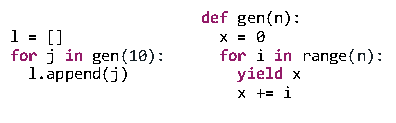
\includegraphics[scale=1.7]{figures/ch6-pypy-example-code}
	\label{fig:pypy_example_code}
}

\subfigure[Optimized trace of the generator loop example]{
	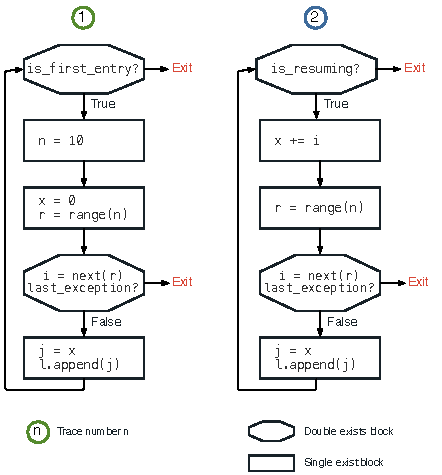
\includegraphics[scale=1.5]{figures/ch6-pypy-example-trace}
	\label{fig:pypy_example_trace}
}
\caption{Generator optimization in PyPy}
\label{fig:pypy_generator_inlining}
\end{figure}

PyPy is the state-of-the-art implementation of Python that implements a meta-tracing JIT compiler for aggressively optimizing Python programs~\cite{bolz.etal09,Rigo2006}.
PyPy is fairly mature and complete compared to ZipPy.

ZipPy on the other hand is more light weight in terms of implementation effort.
It benefits from low-cost speculative type specialization, which is the most critical performance optimization for dynamic languages.
ZipPy does not have to invest or maintain its own compilation infrastructure.
It relies on the underlying Java compiler to JIT compile Python code.
The Java JIT compiler is, in general, more sophisticated and aggressive than the one in PyPy.
Any additional optimizations added to Truffle will automatically benefit our system.

\subsubsection*{PyPy's Generator Optimization}

\begin{table*}
  \begin{center}
  \begin{tabular}{ l r r }
  \toprule
  Benchmark             & Speedup $-$GP & Speedup $+$GP \\
  \midrule
  \textsf{nqueens}      & $0.52$ & $2.36$ \\
  \textsf{euler11}      & $0.72$ & $9.51$ \\
  \textsf{euler31}      & $0.60$ & $1.70$ \\
  \textsf{eratos}       & $2.30$ & $2.63$ \\
  \textsf{lyndon}       & $0.30$ & $6.71$ \\
  \textsf{partitions}   & $0.37$ & $1.58$ \\
  \textsf{pymaging}     & $0.55$ & $1.48$ \\
  \textsf{python-graph} & $0.51$ & $0.92$ \\
  \textsf{simplejson}   & $0.33$ & $1.22$ \\
  \textsf{sympy}        & $0.27$ & $0.36$ \\
  \textsf{whoosh}       & $0.90$ & $2.52$ \\
  \textbf{mean}         & \textbf{$0.55$} & \textbf{$1.95$} \\
  \bottomrule
  \end{tabular}
  \caption{The speedups of ZipPy without and with generator peeling normalized to PyPy3}
  \label{tab:ch6-generator-benchmarks-zippy-vs-pypy}
  \end{center}
\end{table*}

% PyPy inlining stuff
PyPy also supports a generator optimization that primarily targets simple generator functions in its recent releases.
Figure~\ref{fig:pypy_example_code} shows an example generator loop (left) that consumes a simple generator function (right).
We use this example to demonstrate PyPy's optimization.
PyPy is able to trace the execution of the loop and compiles it into machine code.
The trace compiler inlines the implicit call to the generator's \texttt{\_\_next\_\_} method into the loop body.
It does so by constant folding the \texttt{last\_instruction} pointer on the generator frame, which stores the suspended program location in the generator.
The subsequent compiler optimizations convert the \emph{yield} operation to a direct jump.
However, generator frame accesses are not fully optimized, since its allocation happens outside the trace and cannot be seen by the JIT compiler.

PyPy's trace compiler compiles linear execution paths into machine code.
Different iterations of a generator loop are likely to be compiled into different traces.
Figure~\ref{fig:pypy_example_trace} illustrates two different traces the compiler generates for our example.
We simplified the intermediate representation format in PyPy's trace to make it more readable.
The first iteration of the loop goes into trace one; the remaining iterations execute in trace two.
More complicated control structures and multiple yields in a generator function introduce more branches in the consuming loop.
The number of traces generated by the compiler increases for more complicated generators.
As a result, the execution of an optimized generator loop has to switch between different traces.
Not only does the trace switching incur slow paths, it also increases instruction cache misses.
Currently more complicated generators are not properly optimized by PyPy.

Generator peeling on the other hand is able to optimize more complicated generators.
ZipPy using the underlying method-based JIT compiler compiles the entire transformed generator loop into machine code, and completely removes overheads incurred by a generator.
Moreover, by analyzing the assembly code produced by both JIT compilers, we found that, even for a simple generator case, Truffle is able to produce more efficient machine code.
Table~\ref{tab:ch6-generator-benchmarks-zippy-vs-pypy} shows the speedups of ZipPy with and without generator peeling, relative to PyPy3 (Python 3).
The overall performance of ZipPy without generator peeling is competitive with PyPy3.
However, by enabling generator peeling, our system outperforms PyPy3 by a factor of two.
